\section{乘积的分布}
\label{sec:rvt-products}

一块矩形木板的长和宽都是随机的，面积$Z=XY$服从什么分布？取最简单的情形：$X,Y$独立且都服从$\operatorname{Unif}(0,1)$。面积也在$(0,1)$中，但它会更偏向小值，因为两个小于$1$的数相乘只会更小。偏多少，要算出来。

\paragraph{直接按原像计算}
事件$XY\leq z$（$0<z<1$）的原像是单位正方形中双曲线$xy=z$下方的部分。$x\leq z$时整段竖线都在原像中；$x>z$时竖线上满足$y\leq z/x$的部分在原像中。于是
\[
 F_Z(z)=z+\int_z^1\frac{z}{x}\,\mathrm{d}x=z-z\ln z .
\]
求导，$1-\ln z-1=-\ln z$，得到
\begin{equation}
 f_Z(z)=-\ln z,\qquad 0<z<1 .
 \label{eq:rvt-uniform-product}
\end{equation}
它在$z\to0$时趋于无穷，但可积。

\paragraph{辅助坐标}
一般情形用上一节的降维办法：补一个坐标，凑成同维可逆变换。取$W=X$，映射$(x,y)\mapsto(w,z)=(x,xy)$在$x\neq0$的区域上一一，逆映射是$x=w$、$y=z/w$。它的Jacobian行列式是
\[
 \det\begin{pmatrix}1&0\\-z/w^{2}&1/w\end{pmatrix}=\frac1w .
\]

要使用这个变换，需要$\mathbb{P}(X=0)=0$，这样去掉直线$x=0$不损失质量。$(X,Y)$有联合密度时这自动成立，因为直线面积为零。由式~\eqref{eq:rvt-multivariate-density}得到$f_{W,Z}(w,z)=f_{X,Y}(w,z/w)/\lvert w\rvert$，再积掉$w$并改记为$x$，就得到下面的公式。

\begin{theorem}[乘积的密度]
\label{thm:rvt-product-density}
设$(X,Y)$有联合密度$f_{X,Y}$，则$Z=XY$有密度
\begin{equation}
 f_Z(z)=\int_{\mathbb{R}}f_{X,Y}\Bigl(x,\frac zx\Bigr)\frac{1}{\lvert x\rvert}\,\mathrm{d}x .
 \label{eq:rvt-product-density}
\end{equation}
若$X$与$Y$独立，被积函数中的$f_{X,Y}(x,z/x)$换成$f_X(x)\,f_Y(z/x)$。
\end{theorem}

因子$1/\lvert x\rvert$可以这样理解。固定$X=x$，$Z$落在$[z,z+\Delta z]$等价于$Y$落在长度为$\Delta z/\lvert x\rvert$的区间里。$x$越接近零，$Z$的同一段小区间要求$Y$变动的范围越大，收集到的质量越多。乘积的密度在零附近常常变大，原因就在这里。

\paragraph{均匀变量的核对}
把$f_X=f_Y=\mathbf{1}_{(0,1)}$代入式~\eqref{eq:rvt-product-density}。被积函数非零要求$0<x<1$且$0<z/x<1$，即$z<x<1$，于是
\[
 f_Z(z)=\int_z^1\frac{\mathrm{d}x}{x}=-\ln z ,
\]
与直接计算的式~\eqref{eq:rvt-uniform-product}一致。支撑是$(0,1)$，归一化为
\[
 \int_0^1(-\ln z)\,\mathrm{d}z=\bigl[z-z\ln z\bigr]_0^1=1 ,
\]
其中用到了$z\ln z\to0$（$z\to0$）。

数值特征也能核对。独立时$\mathbb{E}[XY]=\mathbb{E}[X]\,\mathbb{E}[Y]=1/4$，而由密度计算
\[
 \int_0^1z(-\ln z)\,\mathrm{d}z=\frac14 .
\]
中位数$m$满足$m-m\ln m=1/2$，数值求解得$m\approx0.187$，远小于均值$0.25$：大部分面积都很小，少数接近$1$的面积把均值拉高。

还有一条独立的路径：对正变量，乘积取对数变成和。由第~\ref{sec:rvt-monotone}节，$-\ln X$与$-\ln Y$都服从$\operatorname{Exp}(1)=\operatorname{Gamma}(1,1)$，由定理~\ref{thm:rvt-group-independence}它们独立；按上一节的Gamma封闭性，它们的和$G=-\ln Z$服从$\operatorname{Gamma}(2,1)$，密度$g\mathrm{e}^{-g}$。再对递减变换$Z=\mathrm{e}^{-G}$用式~\eqref{eq:rvt-monotone-density}，$\lvert h'(z)\rvert=1/z$，得到
\[
 f_Z(z)=(-\ln z)\,\mathrm{e}^{\ln z}\cdot\frac1z=-\ln z .
\]
三种算法给出同一个结果。

图~\ref{fig:rvt-product-uniform}(a)画出原像，(b)用模拟样本核对密度。

\paragraph{符号}
输入可正可负时，式~\eqref{eq:rvt-product-density}自动处理符号，只需注意$z/x$的符号随$x$改变。设$X,Y$独立且都服从$\operatorname{Unif}(-1,1)$，密度各为$1/2$。被积函数非零要求$\lvert x\rvert<1$且$\lvert z/x\rvert<1$，即$\lvert z\rvert<\lvert x\rvert<1$，正负两段$x$对称，于是
\[
 f_Z(z)=\frac14\cdot2\int_{\lvert z\rvert}^{1}\frac{\mathrm{d}x}{x}=-\frac12\ln\lvert z\rvert,\qquad 0<\lvert z\rvert<1 .
\]
它是$-\ln z$对折成的偶函数，总积分仍为$1$。

\paragraph{零处的原子}
输入在零处有原子时，辅助坐标的条件$\mathbb{P}(X=0)=0$失效，要把零单独算。乘积为零当且仅当至少一个因子为零：
\[
 \mathbb{P}(XY=0)=\mathbb{P}(X=0)+\mathbb{P}(Y=0)-\mathbb{P}(X=0,\ Y=0) .
\]
其余的质量在$X\neq0$、$Y\neq0$的部分上按式~\eqref{eq:rvt-product-density}计算。

例如一台机器以概率$0.3$停工、产量为零，以概率$0.7$开工、产量占满负荷的比例服从$\operatorname{Unif}(0,1)$，再乘以一个独立的$\operatorname{Unif}(0,1)$的合格率。设$B\sim\operatorname{Bern}(0.7)$、$X'$、$Y$相互独立，$X',Y\sim\operatorname{Unif}(0,1)$，产量$X=BX'$，合格产量$Z=XY$。则$\mathbb{P}(Z=0)=\mathbb{P}(B=0)=0.3$；$B=1$时$Z=X'Y$，所以$Z$在$(0,1)$上的连续部分是$0.7\cdot(-\ln z)$。分布函数是
\[
 F_Z(z)=0.3+0.7\,(z-z\ln z),\qquad 0\leq z<1 .
\]
若对$X$的“密度部分”$0.7\cdot\mathbf{1}_{(0,1)}$直接套用式~\eqref{eq:rvt-product-density}而不另计原子，总质量只有$0.7$。

\begin{BookInlineFigure}
  \centering
  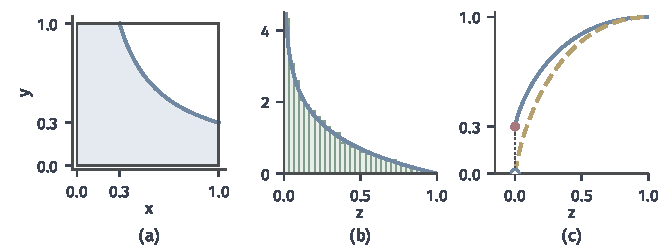
\includegraphics[width=112mm]{figures/07-probability/01-elementary-probability/matplotlib/rvt-product-uniform/figure.pdf}
  \caption{两个独立$\operatorname{Unif}(0,1)$的乘积。(a)浅蓝区域是$XY\leq0.3$的原像，蓝线为双曲线$xy=0.3$，面积$0.3-0.3\ln0.3\approx0.661$。(b)密度$-\ln z$（蓝）与$20000$个模拟样本的直方图（浅绿，种子$13$）。(c)$X$在零处有$0.3$的原子时乘积的分布函数（蓝），红点表示零处的原子，黄色虚线是没有原子时的$z-z\ln z$。}
  \label{fig:rvt-product-uniform}
\end{BookInlineFigure}

乘积的公式与和的公式结构相同，都是“补一个坐标、积掉它”；不同的是乘积的变换在$x=0$处不可逆，所以多了$1/\lvert x\rvert$这个因子，也多了对零处原子的检查。
